\section{Second-order Cone Problems} % (fold)
\label{sec:second_order_cone_problems}

\begin{definition}[cone]
	Set of points $C\in \mathbb{R}^n$ is a cone iff
	\[
\alpha\v{x}\in C\;\;\;\text{if }\v{x}\in C\;\;\;\forall \alpha\ge0
	\]
\end{definition}

\begin{definition}[convex cone]
	C is a convex cone if
	\[
\alpha\v{x}\in C \;\;\;\forall \alpha\ge0 \;\text{ and } \theta_1,\theta_2\ge 0
	\]
	Then 
	\[
\theta_1\v{x}_1+\theta_2\v{x}_2 \in C
	\]
\end{definition}

\begin{example}
	\[C = \{(x, y)\;|\;y\ge 0\}\]
	This cone has a feasible region of all region above x-axis.
\end{example}

\begin{definition}[Polyhedron cone]
	\[
\text{Polyhedron: }\{\v{x}\;|\; A\v{x}-\v{b} \}
	\]
\end{definition}

\begin{definition}[Ellipsoidal cone]
	This is the kind of cone we are going to concern the most. Recall that
	\[
\v{x}^\top P\v{x}+\v{q}^\top \v{x}+r\le 0,\;\;P\succ0
	\]
	Defines a ellipsoid. Consider
	\begin{align*}
		\|A\v{x}+b\|_2^2 &\le c^2 \\
		\v{x}^\top A^\top A\v{x}+2\v{b}^\top A\v{x}+\v{b}^\top\v{b}-c^2&\le 0
	\end{align*}
	Then \[
\{(\v{x}, t)\;|\;\|A\v{x}+\v{b}t\|_2\le ct\}
	\] is an ellipsoidal cone.
\end{definition}

\begin{remark}[Special case of Ellipsoidal cone (second-order cone)]
	Consider a second-order cone in $\mathbb{R}^3$
	\[
\{(\v{x}_1,\v{x}_2,t)\;|\;\sqrt{\v{x}_1^2+\v{x}_2^2}\le t\}
	\]
	is the "ice cream cone" because it looks like a ice cream cup.
\end{remark}

\begin{definition}[SOCP]
\begin{align*}
	&\min \v{q}^\top\v{x}\\
	s.t.\;\;\;&\|A_i\v{x}+b_i\|_2\le \v{c}_i^\top\v{x}+\v{d}_i \;\;\;i=1,2,\cdots,m
\end{align*}
Is a SOCP. It is a program with constraints that takes the form of a cone.
\end{definition}

\begin{example}
	\begin{align*}
		\min_x\sum_{i=1}^m\|A_i\v{x}-\v{b}_i\|_2
	\end{align*}
	Can be formulated into a SOCP:
	\begin{align*}
		&\min_x\sum_{i=1}^m\|A_i\v{x}-\v{b}_i\|_2\\
		=&\min_{x, y_i, \|A_i\v{x}-\v{b}_i\|_2 = y_i}\sum_{i=1}^my_i& \text{relax the equality into inequality}\\
		=&\min_{x, y_i, \|A_i\v{x}-\v{b}_i\|_2 \le y_i}\sum_{i=1}^my_i
	\end{align*}
\end{example}

\begin{example}[Facility Location Problem]
		Say we want to place a facility (playground or ER, etc.) and we want this facility to be close to people.\\
	\center
	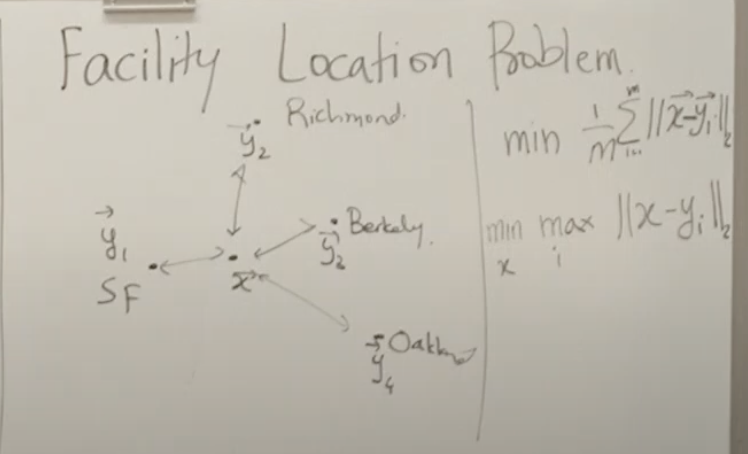
\includegraphics{img/FLP.png}
\end{example}

\begin{example}[Trilateration/GPS]
	A packet is transmitted at $t_i^T$ and received at $t_i^R$ with an offset $\delta$ such that
	\[
t_i^{\text{true}} = t_i^R+\delta
	\]
	\begin{itemize}
		\item Time of flight $f_i = t_i^{\text{true}} - t_i^T = t_i^R+\delta- t_i^T = \Delta_i+\delta$
		\item Distance $cf_i = c \Delta_i+c \delta = \|\v{x}-\v{q}_i\|_2$
	\end{itemize}
	Where c = the speed of light, x is the current location and q is the satellite location. We use 4 satellites, sqare all the equations, and substract them from the equation of satellite \#4.
	\begin{align*}
		\|x-q_4\|_2^2 - \|x-q_1\|_2^2&=x^\top x-x^\top x+0x+const\\
		2(q_4-q)^\top x+2c^2(\Delta_4- \Delta_1)\delta &= c^2(\Delta_1^2- \Delta_4^2)+\|q_4\|_2^2-\|q_1\|_2^2
	\end{align*}
	But what if instead of four satellites, we only have three satellites? We can solve this via SOCP by constructing optimization problem
	\begin{align*}
	&\min \delta\\
	s.t.\;\;\;&2(q_3-q_1)^\top x+2c^2(\Delta_3- \Delta_1)\delta = c^2(\Delta_1^2- \Delta_3^2)+\|q_3\|_2^2-\|q_1\|_2^2\\
	&2(q_3-q_2)^\top x+2c^2(\Delta_3- \Delta_2)\delta = c^2(\Delta_2^2- \Delta_3^2)+\|q_3\|_2^2-\|q_2\|_2^2\\
	&\|x-q_3\|_2=c \Delta_3+c \delta
	\end{align*}
\end{example}

% section second_order_cone_problems (end)